\documentclass[12pt]{article}

\usepackage[T1]{fontenc}
\usepackage[utf8]{inputenc}
\usepackage[russian]{babel}

\usepackage{amsmath}
\usepackage{float}
\usepackage{tabularx}

% page margin
\usepackage[top=2cm, bottom=2cm, left=2cm, right=2cm]{geometry}

\usepackage{graphicx}

\usepackage{fancyhdr}
\pagestyle{fancy}
% modifying page layout using fancyhdr
\fancyhf{}
\renewcommand{\sectionmark}[1]{\markright{\thesection\ #1}}
\renewcommand{\subsectionmark}[1]{\markright{\thesubsection\ #1}}

\rhead{\fancyplain{}{\rightmark }}
\cfoot{\fancyplain{}{\thepage }}

\renewcommand{\arraystretch}{1.3}

\begin{document}

\begin{figure}[!ht]
	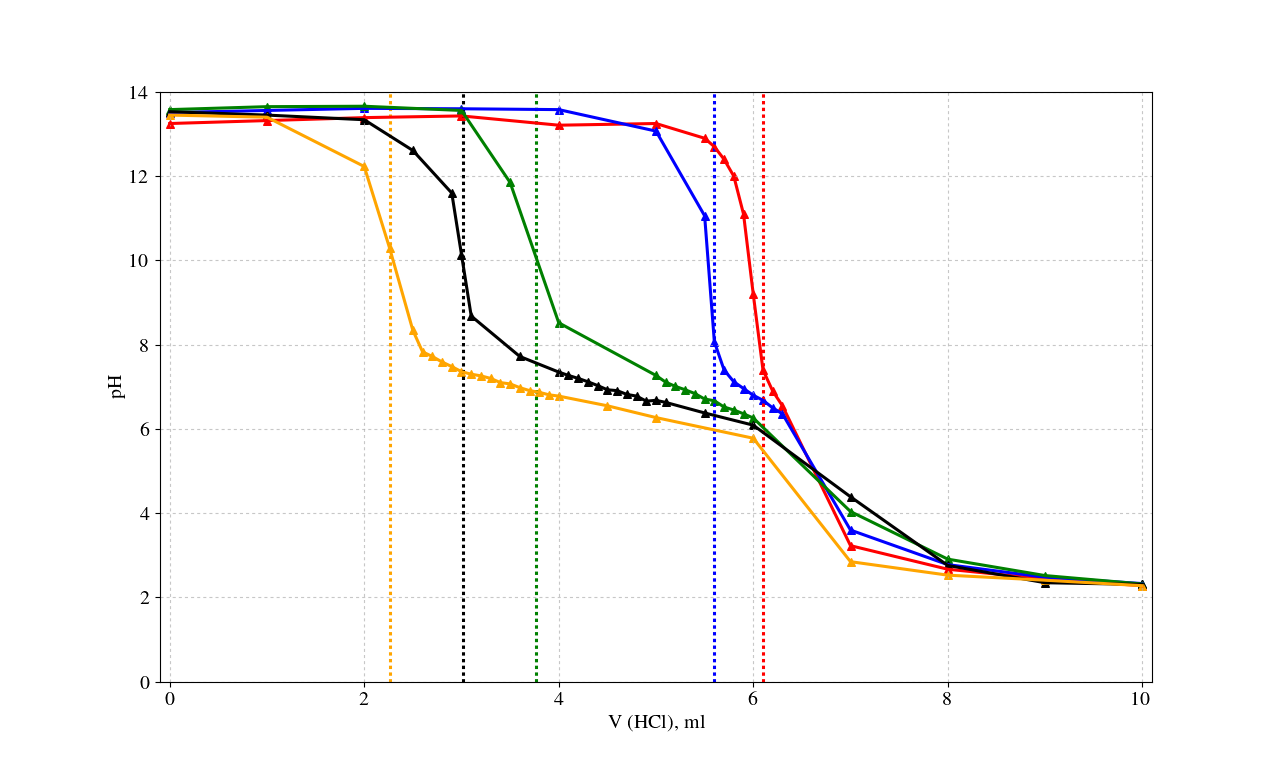
\includegraphics[width = \linewidth]{../titrio.png}
	\caption{Кривые титрования}
\end{figure}

\begin{gather}
		A = \frac{C_0 (\textup{ПВА}) - \left( C_0 (NaOH) - C(NaOH) \right)}{C_0 (\textup{ПВА})} \notag 
\end{gather}

\begin{table}[!ht]
\begin{center}
\caption{}
\begin{tabular}{cccccc}
	\hline
	t, мин & V(HCl), мл & C(NaOH), M & $t^\prime$, M $\cdot$ мин & A & -ln A  \\
	\hline
	0 & -- & 0.0030 & -- & -- & -- \\
	7.0 & 6.1 & 0.017 & 0.163 & 0.708 & -0.345 \\ 
	14.0 & 5.6 & 0.015 & 0.277 & 0.682 & -0.383 \\
	21.0 & 3.8 & 0.011 & 0.371 & 0.578 & -0.549 \\
	28.0 & 3.0 & 0.009 & 0.443 & 0.532 & -0.631 \\ 
	35.0 & 2.3 & 0.007 & 0.499 & 0.483 & -0.728 \\
	\hline
\end{tabular}
\end{center}
\end{table}

\begin{figure}[!ht]
	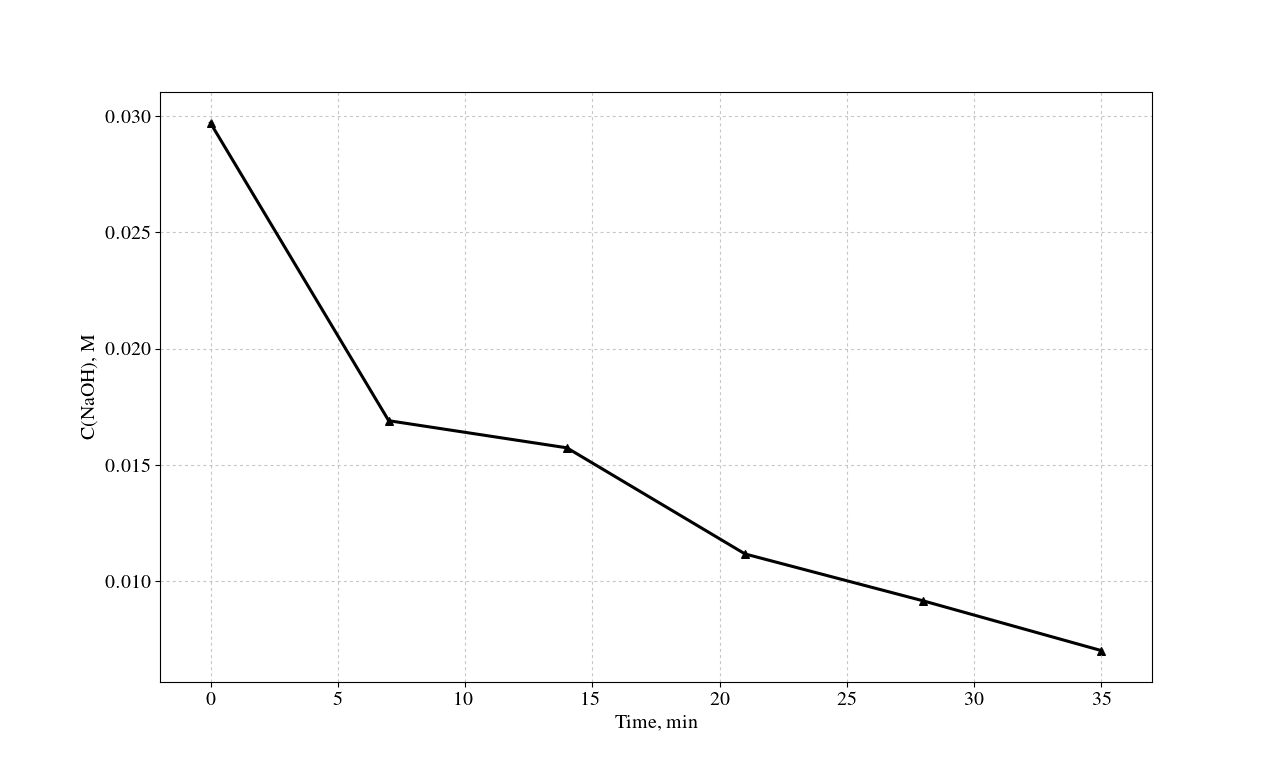
\includegraphics[width = \linewidth]{../naoh.png}
	\caption{Зависимость концентрации щелочи от времени}
\end{figure}

\begin{figure}[!ht]
	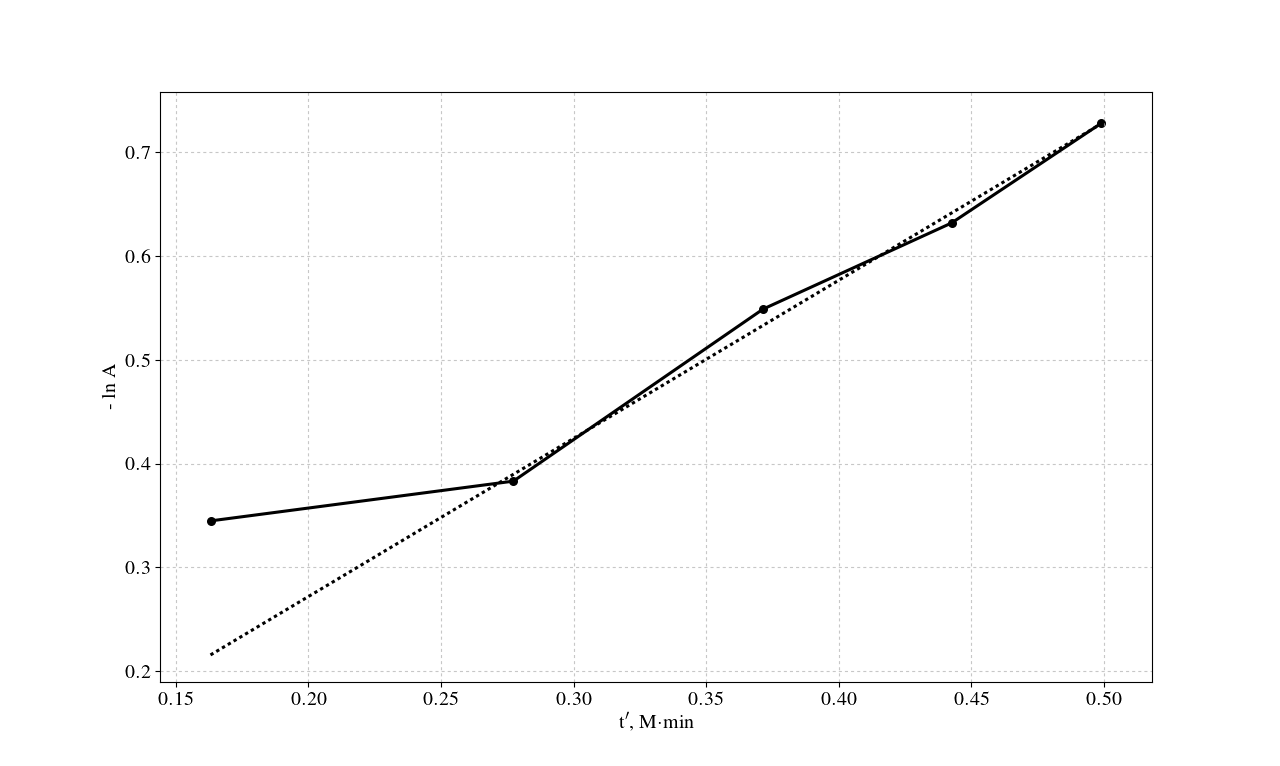
\includegraphics[width = \linewidth]{../kinetic.png}
	\caption{Кинетическая кривая}
\end{figure}

По наклону кинетической кривой определяем константу гидролиза: $k = 1.52 \, M^{-1} \cdot min^{-1}$. Индукционный период реакции -- 14 мин.

\end{document}
